\documentclass[Markos_Delaportas_1316.tex]{subfiles}

\begin{document}

    \section{Ideal Over-the-Air Computation Baseline}
    Before introducing the practical impairments inherent to wireless channels, such as
    \gls{isi}, multipath fading, and time synchronization errors, it is essential to
    establish a baseline model of \gls{ota} computation under ideal
    conditions. The foundational premise of \gls{ota} computing is its ability to reduce
    the communication latency of data aggregation from $\mathcal{O}(K)$ to
    $\mathcal{O}(1)$ by allowing $K$ devices to transmit simultaneously
    \cite{sahin_survey_2023}. 
    
    In this idealized scenario, the wireless medium is assumed to be perfectly
    synchronized, lacking frequency-selective fading, and corrupted solely by \gls{awgn}.
    This chapter aggregates the mathematical formulation,
    algorithmic MATLAB modeling, block-level Simulink architecture, and GNU Radio
    flowgraphs that demonstrate this ideal, unimpaired baseline. Establishing this
    benchmark is critical for quantifying the exact degradation caused by physical channel
    constraints in subsequent chapters.

    \subsection{Mathematical Formulation of the Ideal Channel}
    Consider a distributed wireless sensor network consisting of $K$ \gls{ed}s
    transmitting local analog values to a central \gls{fc}. Let $x_k(t)$ denote
    the continuous-time, real-valued signal transmitted by the $k$-th device. For analog
    \gls{ota} computation, uncoded \gls{pam} is widely
    considered the optimal transmission scheme, as it linearly maps the sensor readings
    directly to the amplitude of the transmitted waveform \cite{goldenbaum_robust_2013,
    zhu_one-bit_2021}.

    In an ideal \gls{mac}, we assume perfect \gls{csi} at the transmitters, which allows 
    for flawless pre-equalization of phase shifts
    and path loss attenuation. Consequently, the electromagnetic waves superimpose
    perfectly at the receiving antenna of the \gls{fc}. The received baseband signal $y(t)$ is
    mathematically expressed as the linear sum of the transmitted signals plus noise:
    \begin{equation}
        y(t) = \sum_{k=1}^{K} x_k(t) + n(t) \label{eq:mac_sum}
    \end{equation}
    where $n(t) \sim \mathcal{N}(0, \sigma^2)$ represents the \gls{awgn} with zero mean and
    variance $\sigma^2$. Because there is no multipath delay spread in this baseline
    model, the channel impulse response is effectively a Dirac delta function $h(t) =
    \delta(t)$. This implies that the current symbol is entirely unaffected by past or
    future symbols, resulting in zero \gls{isi}. To extract the arithmetic average of the
    $K$ sensor readings, the \gls{fc} simply applies a post-processing scaling factor of $1/K$
    to the received aggregated signal $y(t)$.

    \subsection{MATLAB Simulation and Code Analysis}
    To validate this superposition principle, the ideal environment can be modeled using MATLAB. 
    The following
    script generates normally distributed simulated sensor readings, aligns them perfectly
    in time, and adds \gls{awgn} to emulate the ideal \gls{mac}.

    \begin{lstlisting}[style=Matlab-editor, caption={MATLAB script for ideal OTA computation aggregation.}, label={lst:ideal_ota}]
        % Ideal OTA Computation Simulation
        K = 3;                  % Number of sensors
        N = 1000;               % Number of samples
        SNR_dB = 20;            % Signal-to-Noise Ratio

        % Generate random temperature readings around 27 degrees
        X = 27 + randn(K, N); 

        % The Air acts as an ideal adder (MAC Superposition)
        Ideal_Sum = sum(X, 1);

        % Add AWGN
        Received_Signal = awgn(Ideal_Sum, SNR_dB, 'measured');

        % Calculate the Fusion Center Average
        Estimated_Average = Received_Signal / K;

        % Display Mean Squared Error (MSE)
        MSE = immse(Estimated_Average, mean(X, 1)); fprintf('Ideal Baseline MSE at %d dB SNR: %f\n', SNR_dB, MSE);
    \end{lstlisting}

    While Listing~\ref{lst:ideal_ota} demonstrates the fundamental principle in its unadulterated form, 
    practical wireless systems necessitate pulse shaping to satisfy spectral constraints and facilitate 
    signal recovery. Consequently, a more physically realistic model incorporates matched \gls{rc} 
    filtering at both the transmitter and receiver. This architectural refinement introduces 
    additional degrees of freedom—namely, the \gls{sps} parameter and the roll-off 
    factor ($\alpha$)—which materially influence system performance. The enhanced implementation is presented 
    in Listing~\ref{lst:ideal_ota_rc}.

    \begin{lstlisting}[style=Matlab-editor, caption={MATLAB script for OTA computation aggregation using the \gls{rc} filter.}, label={lst:ideal_ota_rc}]
        txUpSamped = upsample(X', sps_val); % phase may need to be set

        % Raised Cosine Filter
        rcFilter = rcosdesign(aleph, span, sps_val, "sqrt");

        rx_agg_signal = zeros(N * sps_val + length(rcFilter) - 1, 1);

        for k = 1:K
            rx_agg_signal = rx_agg_signal + conv(txUpSamped(:,k), rcFilter(:));
        end

        Received_Signal = awgn(rx_agg_signal, current_snr, 'measured');

        matchedSignal = conv(Received_Signal, flipud(rcFilter(:)), 'same');

        rxMatched = downsample(matchedSignal, sps_val);

        start_idx = floor(span/2); stop_idx = floor(span/2) + mod(span,2) + 1;

        % Truncate edges to avoid filter transient errors
        Estimated_Average = rxMatched(start_idx:end-stop_idx, :) / K;

        % Calculate and store MSE in the matrix
        mse_results(snr_idx, a_idx) = immse(Estimated_Average', mean(X, 1));
    \end{lstlisting}

    % As demonstrated by the script, when synchronization is perfect, the MSE is strictly a
    % function of the \gls{awgn} variance. When however trying to implement a scenario that is closer
    % to a real world usecase, it appears to be necessary to interject a filter pair like the
    % raised cosine filter. In order for this to be accomplished, a matched root raised cosine 
    % filter shall be inserted on each end of channel and by doing that, more degrees of freedom 
    % shall be taken into account, like \gls{sps} and \gls{rof}. In diagram \ref{plt:rcOTAmse}
    % the curve can be seen where in diagram \ref{plt:idealOTAmse} the ideal \gls{mse} can
    % be shown. 

    % As demonstrated by the script's execution, when synchronization is mathematically
    % perfect, the computational accuracy relies entirely on the noise floor. The \gls{mse}
    % of the estimation is strictly a function of the \gls{awgn}
    % variance scaled by the number of transmitting devices, mathematically bounded as
    % $\text{MSE} \propto \sigma^2/K^2$. This demonstrates that in an ideal \gls{ota}
    % scenario, increasing the number of sensors actually improves the accuracy of the
    % computed average due to the noise-averaging effect \cite{sahin_survey_2023,
    % cao_optimized_2022}.

    Computational execution of the aforementioned algorithms reveals a critical distinction between the 
    idealized and practical regimes. When temporal synchronization is mathematically perfect and no filtering 
    is applied, the estimation accuracy is entirely governed by the noise floor; the \gls{mse} exhibits 
    a direct proportionality to the \gls{awgn} variance and inverse quadratic scaling with the number of 
    transmitting sensors. Mathematically, this relationship is expressed as $\text{MSE} \propto \sigma^2/K^2$, 
    which demonstrates the fundamental advantage of cooperative multi-device aggregation \cite{sahin_survey_2023,
    cao_optimized_2022}. Conversely, when pulse shaping filters are incorporated into the transmission chain, 
    the interplay between symbol timing parameters (\gls{sps}) and spectral efficiency (\gls{rof}) introduces 
    measurable deviation from the ideal theoretical bound.

    \begin{center}
        \begin{minipage}{.45\textwidth}
            \begin{tikzpicture}
                \begin{axis}[
                    title={\textsf{Ideal}},
                    xlabel={SNR (dB)}, ylabel={MSE},
                    ymode=log, grid=major,
                    legend pos=north east,
                ]
                    \addplot[
                        color=blue,
                        mark=square,
                        thick
                    ] table[x=SNR_dB, y=MSE] {data/IdealBaseline_MSE.txt};
                    
                    \addlegendentry{Ideal}
                \end{axis}
            \end{tikzpicture}
            % \caption{\textsf{}}
            \label{plt:idealOTAmse}
        \end{minipage}
        \begin{minipage}{.45\textwidth}
            \begin{tikzpicture}
                \begin{axis}[
                    title={\textsf{RC-Filtered}},
                    xlabel={SNR (dB)}, ylabel={MSE},
                    ymode=log, grid=major,
                    legend pos=north east,
                ]
                    \addplot[
                        color=red,
                        mark=*,
                        thick,
                        restrict expr to domain={\thisrow{aleph_array}}{0.49:0.51} 
                    ] table[x=SNR_dB, y=mse_results] {data/MSEvsSNR_10sps.txt};

                    \addlegendentry{sps=$10^1$, $\alpha=0.5$}

                \end{axis}
            \end{tikzpicture}
            % \caption{\textsf{}}
            \label{plt:rcOTAmse}
        \end{minipage}
    \end{center}

    Figure~\ref{plt:idealOTAmse} presents the theoretical performance floor, wherein the \gls{mse} 
    is a function solely of \gls{awgn} variance. In contrast, Figure~\ref{plt:rcOTAmse} illustrates 
    the performance envelope when matched Raised Cosine filters are deployed at both transmitter 
    and receiver, with \gls{sps} and \gls{rof} held constant. Despite the introduction of filtering, 
    the channel remains free of multipath distortion and timing misalignment, ensuring that noise 
    contributions remain the dominant performance-limiting factor.

    \begin{figure}[htbp]
        \centering

        \begin{luacode*}
            local sps_data = {
                {val = "10", label = "1 \\times 10^1"},
                {val = "20", label = "2 \\times 10^1"},
                {val = "30", label = "3 \\times 10^1"},
                {val = "40", label = "4 \\times 10^1"},
                {val = "50", label = "5 \\times 10^1"},
                {val = "60", label = "6 \\times 10^1"},
                {val = "70", label = "7 \\times 10^1"},
                {val = "80", label = "8 \\times 10^1"},
                {val = "90", label = "9 \\times 10^1"},

                {val = "100", label = "1 \\times 10^2"},
                {val = "200", label = "2 \\times 10^2"},
                {val = "300", label = "3 \\times 10^2"},
                {val = "400", label = "4 \\times 10^2"},
                {val = "500", label = "5 \\times 10^2"},
                {val = "600", label = "6 \\times 10^2"},
                {val = "700", label = "7 \\times 10^2"},
                {val = "800", label = "8 \\times 10^2"},
                {val = "900", label = "9 \\times 10^2"},
            }

            local angle = 0 -- in degrees

            tex.print("\\begin{animateinline}[controls, autoplay, loop]{1.5}")
            for i, sps in ipairs(sps_data) do
                
                if i > 1 then
                    tex.print("\\newframe")
                end

                tex.print("\\begin{tikzpicture}")
                tex.print("\\begin{axis}[")
                tex.print("    title={Over-The-Air Computing MSE Profile (sps = $" .. sps.label .. "$)},")
                tex.print("    xlabel={SNR (dB)},")
                tex.print("    ylabel={Roll-off factor ($\\alpha$)},")
                tex.print("    zlabel={MSE},")
                tex.print("    zmode=log,")
                tex.print("    zmin=0.1, zmax=8000,") 
                tex.print("    view={" .. 45 + angle % 135 .. "}{30},")
                tex.print("    grid=major,")
                tex.print("    colorbar,")
                tex.print("    colormap name=viridis")
                tex.print("]")
                
                -- Ensure this path perfectly matches your MATLAB output
                tex.print("\\addplot3[surf] table[x=SNR_dB, y=aleph_array, z=mse_results] {data/MSEvsSNR_" .. sps.val .. "sps.txt};")
                
                tex.print("\\end{axis}")
                tex.print("\\end{tikzpicture}")

                angle = angle + 5
            end
            tex.print("\\end{animateinline}")
        \end{luacode*}

        \caption{Interactive OTA computing animation demonstrating the architectural impact of Samples Per Symbol ($sps$) scaling.}
        \label{fig:ota_mse_morph}
    \end{figure}

    % REPHRASED SECTION: Observation about SPS scaling
    A particularly noteworthy observation emerges from parametric analysis of the animation in Figure~\ref{fig:ota_mse_morph}: 
    while increasing \gls{sps} generally yields marginal improvements in \gls{mse} performance across the SNR range examined, 
    this enhancement asymptotically approaches a limit and does not constitute convergence toward the theoretical ideal baseline 
    (absent pulse shaping). This behavior underscores a fundamental trade-off inherent to practical pulse-shaping implementations: 
    enhanced spectral efficiency through reduced \gls{sps} incurs amplified inter-symbol interference, whereas elevated oversampling 
    ratios improve timing robustness at the cost of increased computational complexity and memory consumption.

    % write a paragraph about the observation of the eye and constellation diagrams that are to be inserted below
    The eye and constellation diagrams provide valuable insights into the behavior of the ideal OTA system under different 
    SPS configurations. As the number of samples per symbol increases, the eye opening widens, indicating reduced inter-symbol 
    interference and improved signal integrity. Similarly, the constellation points become more distinct and well-separated, 
    reflecting better performance in terms of error probability and overall system reliability.

    \begin{figure}[htbp]
        \centering

        \begin{subfigure}[b]{0.39\textwidth}
            \centering
            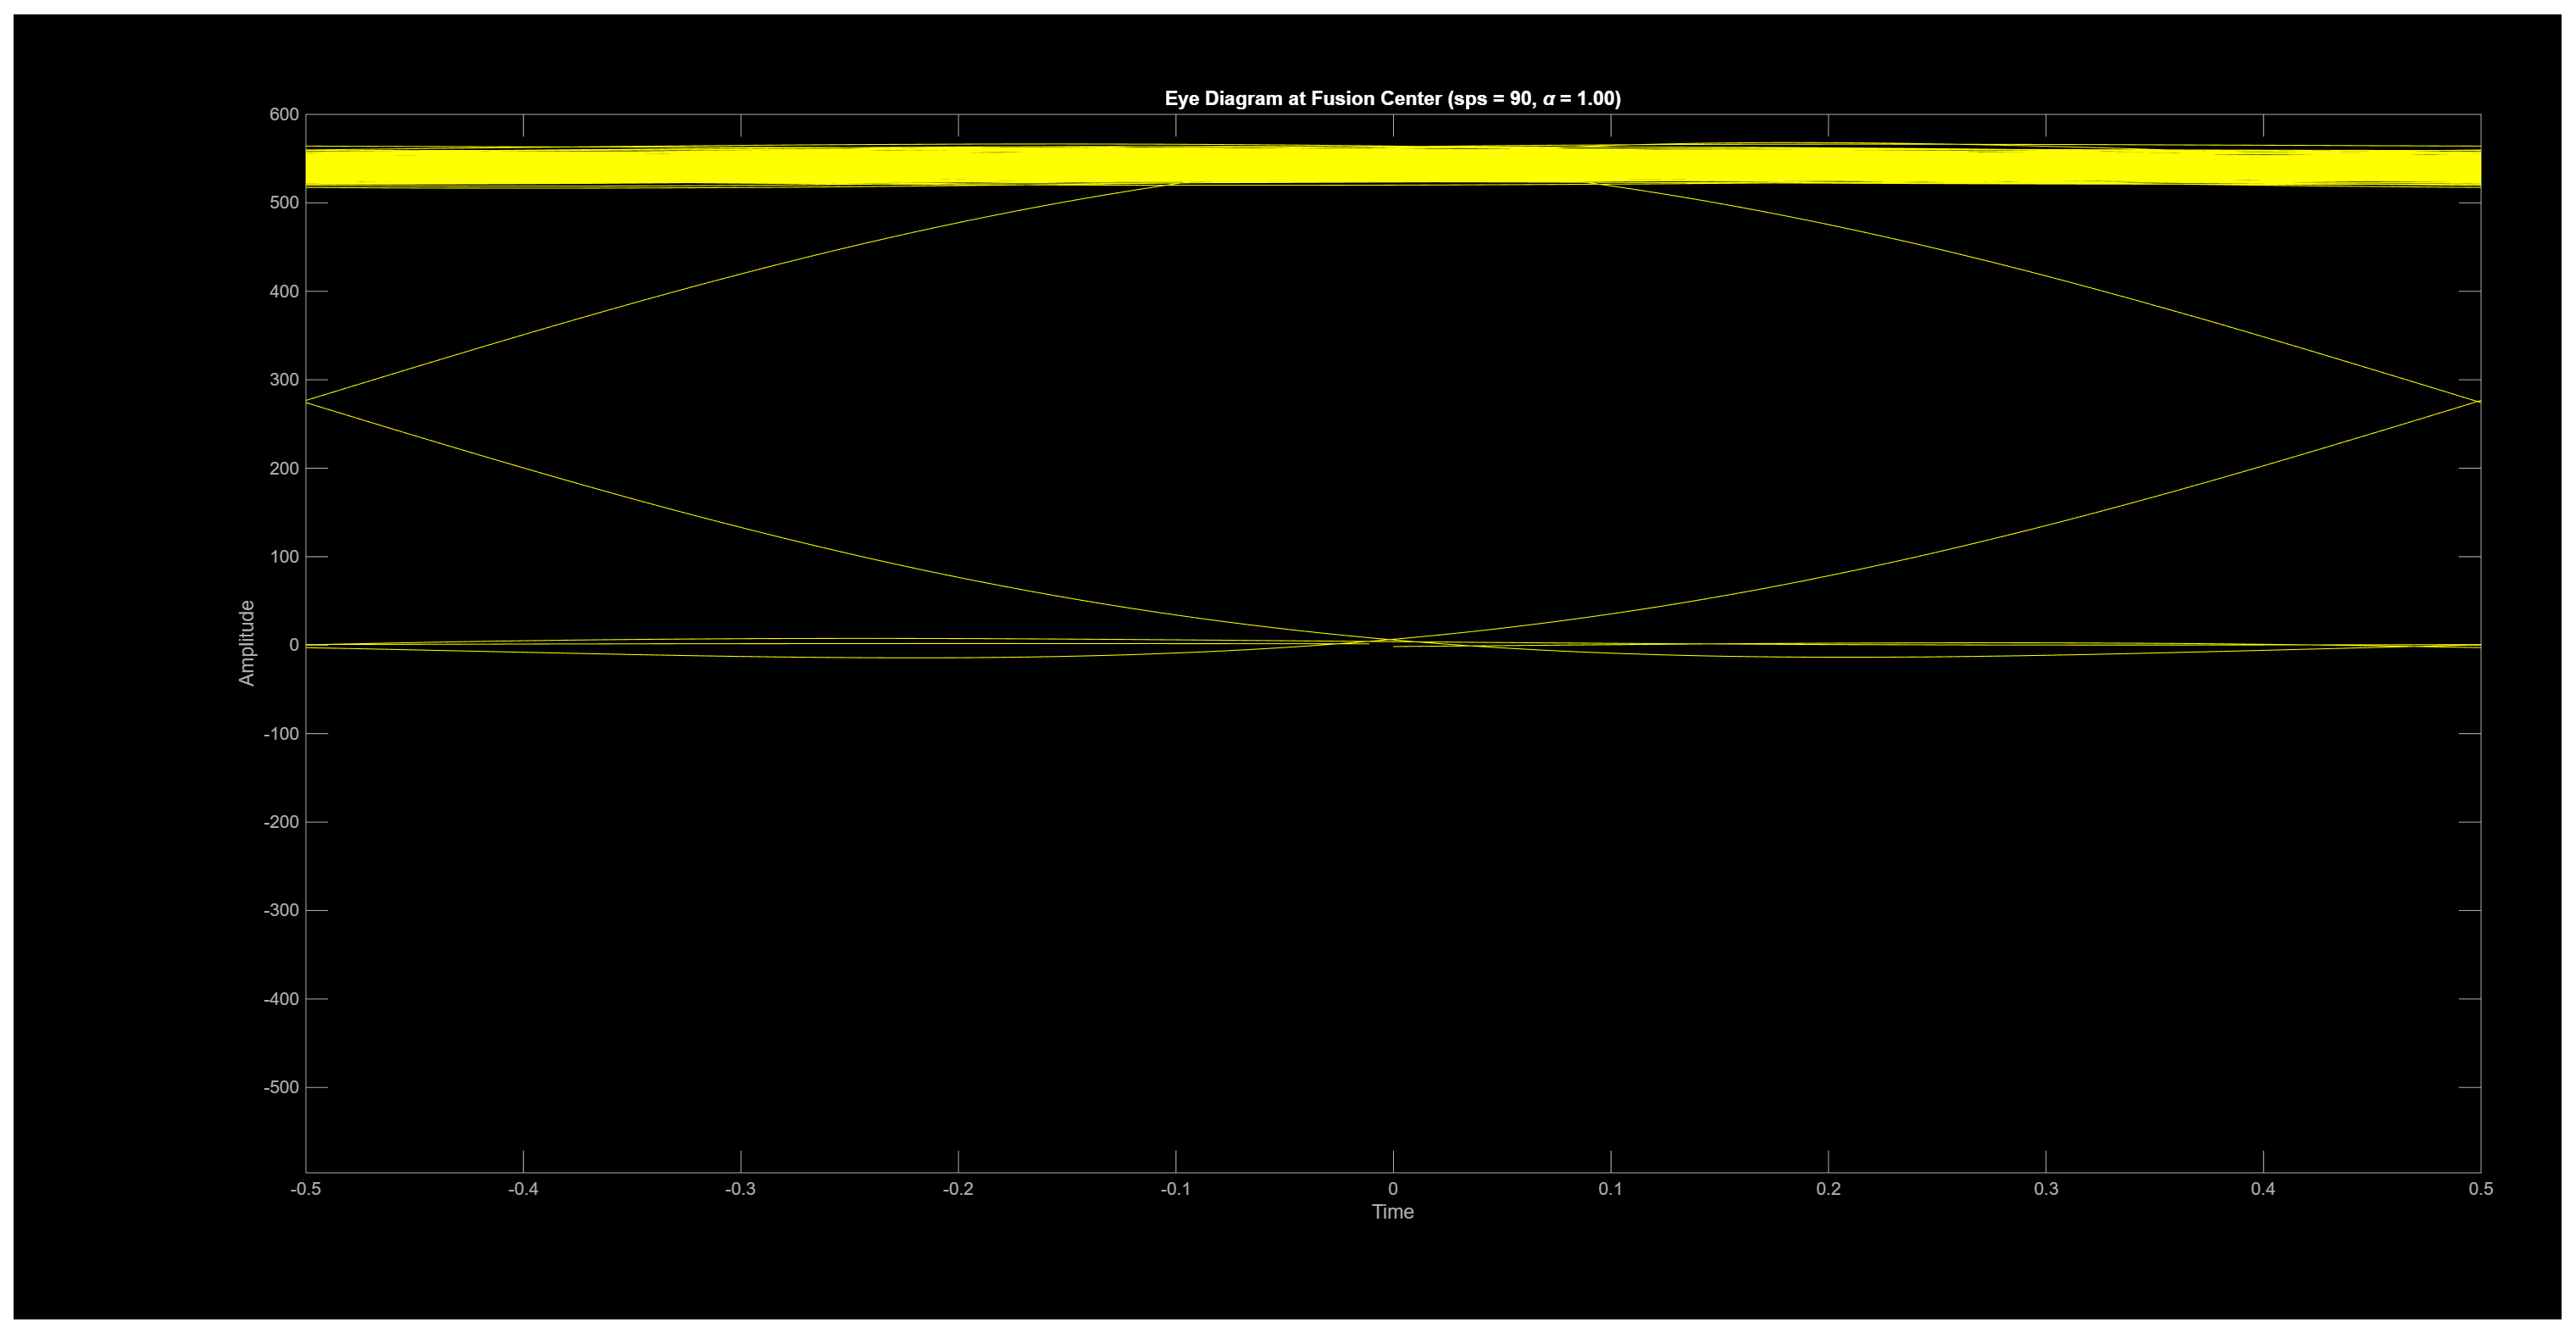
\includegraphics[width=\textwidth]{data/fusion_eye_90sps.eps}
            \caption{Eye diagram at 90 SPS}
            \label{fig:fusion_eye_90sps}
        \end{subfigure}
        
        \hfill

        \begin{subfigure}[b]{0.39\textwidth}
            \centering
            \begin{tikzpicture}
                \begin{axis}[
                    title={Constellation Diagram at Fusion Center},
                    xlabel={In-Phase (I)},
                    ylabel={Quadrature (Q)},
                    ymin=-1, ymax=1, % Lock the Y-axis since Q is always 0
                    grid=major,
                    width=\textwidth,
                    height=0.4\textwidth
                ]
                    % Use 'only marks' to create a scatter plot instead of lines
                    \addplot[
                        only marks,
                        mark=*,
                        mark size=1.5pt,
                        color=blue,
                        opacity=0.4 % Adding opacity shows density where points overlap
                    ] table[x=I_Data, y=Q_Data] {data/fusion_constellation_90sps.txt};
                \end{axis}
            \end{tikzpicture}

            \caption{Native scatter plot of the real-valued symbol constellation at 90 SPS.}
            \label{fig:fusion_constellation_90sps}
        \end{subfigure}

        \caption{Signal integrity analysis at the Fusion Center. Top: Eye diagram illustrating Inter-Symbol Interference bounds. Bottom: Native scatter plot of the real-valued symbol constellation.}
        \label{fig:signal_integrity}
    \end{figure}

    \subsection{MATLAB Simulink Architecture}
    Transitioning from raw code to a block-level architecture, MATLAB Simulink provides a
    clear visual representation of the feedforward ideal system. In this model, the
    transmitters use standard \gls{pam} without the need for
    complex feedback loops or equalizers.

    \begin{figure}[htpb]
        \centering
        \includegraphics[width=\linewidth]{flowgraphs/idealOTA_simulink.pdf}        
        \caption{Simulink block diagram representing the ideal OTA computation network over an \gls{awgn} channel.}
        \label{fig:idealOTA_simulink}
    \end{figure}

    To bridge the gap between theory and practical system implementation, an enhanced model incorporating 
    Raised Cosine pulse shaping is presented in Figure~\ref{fig:idealOTA_simulink_rc}. This architecture 
    employs matched filtering pairs at both transmission and reception stages, enabling quantitative assessment 
    of performance degradation attributable to finite symbol-rate sampling and spectral roll-off constraints.

    \begin{figure}[htpb]
        \centering
        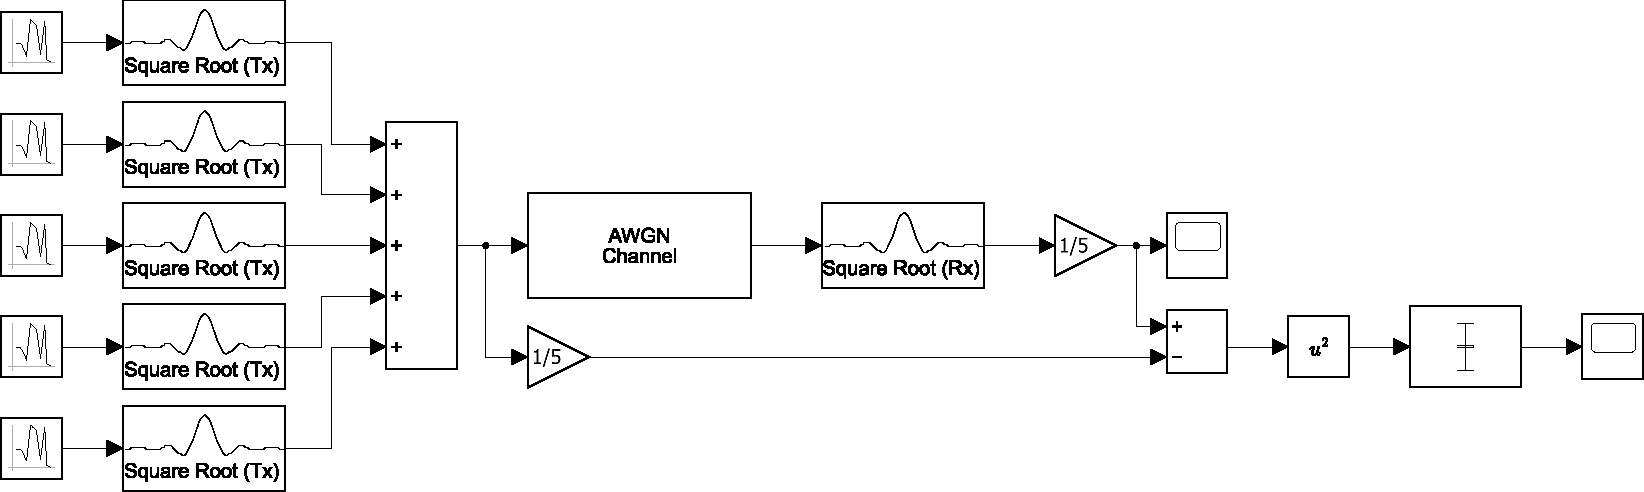
\includegraphics[width=\linewidth]{flowgraphs/idealOTA_simulink_rc.pdf}        
        \caption{Simulink block diagram representing the ideal OTA computation network over an \gls{awgn} channel.}
        \label{fig:idealOTA_simulink_rc} 
    \end{figure}

    Inspection of the \gls{mse} calculation scope output demonstrates the quantitative deviation between 
    the recovered aggregated estimate and the theoretical true value, reflecting the stochastic influence 
    of the additive Gaussian noise. It is noteworthy that practical over-the-air computation mandates 
    time-varying transmission (as opposed to static constant-valued signals), as pulse shaping through 
    \gls{fir} filtering inherently requires symbol-rate sampling and subsequent interpolation. Consequently, 
    systems employing matched filter pairs necessitate carefully synchronized symbol generation to avoid 
    spurious transient responses.

    \begin{figure}[h]
        \centering
        \begin{subfigure}{0.39\textwidth}
            \centering
            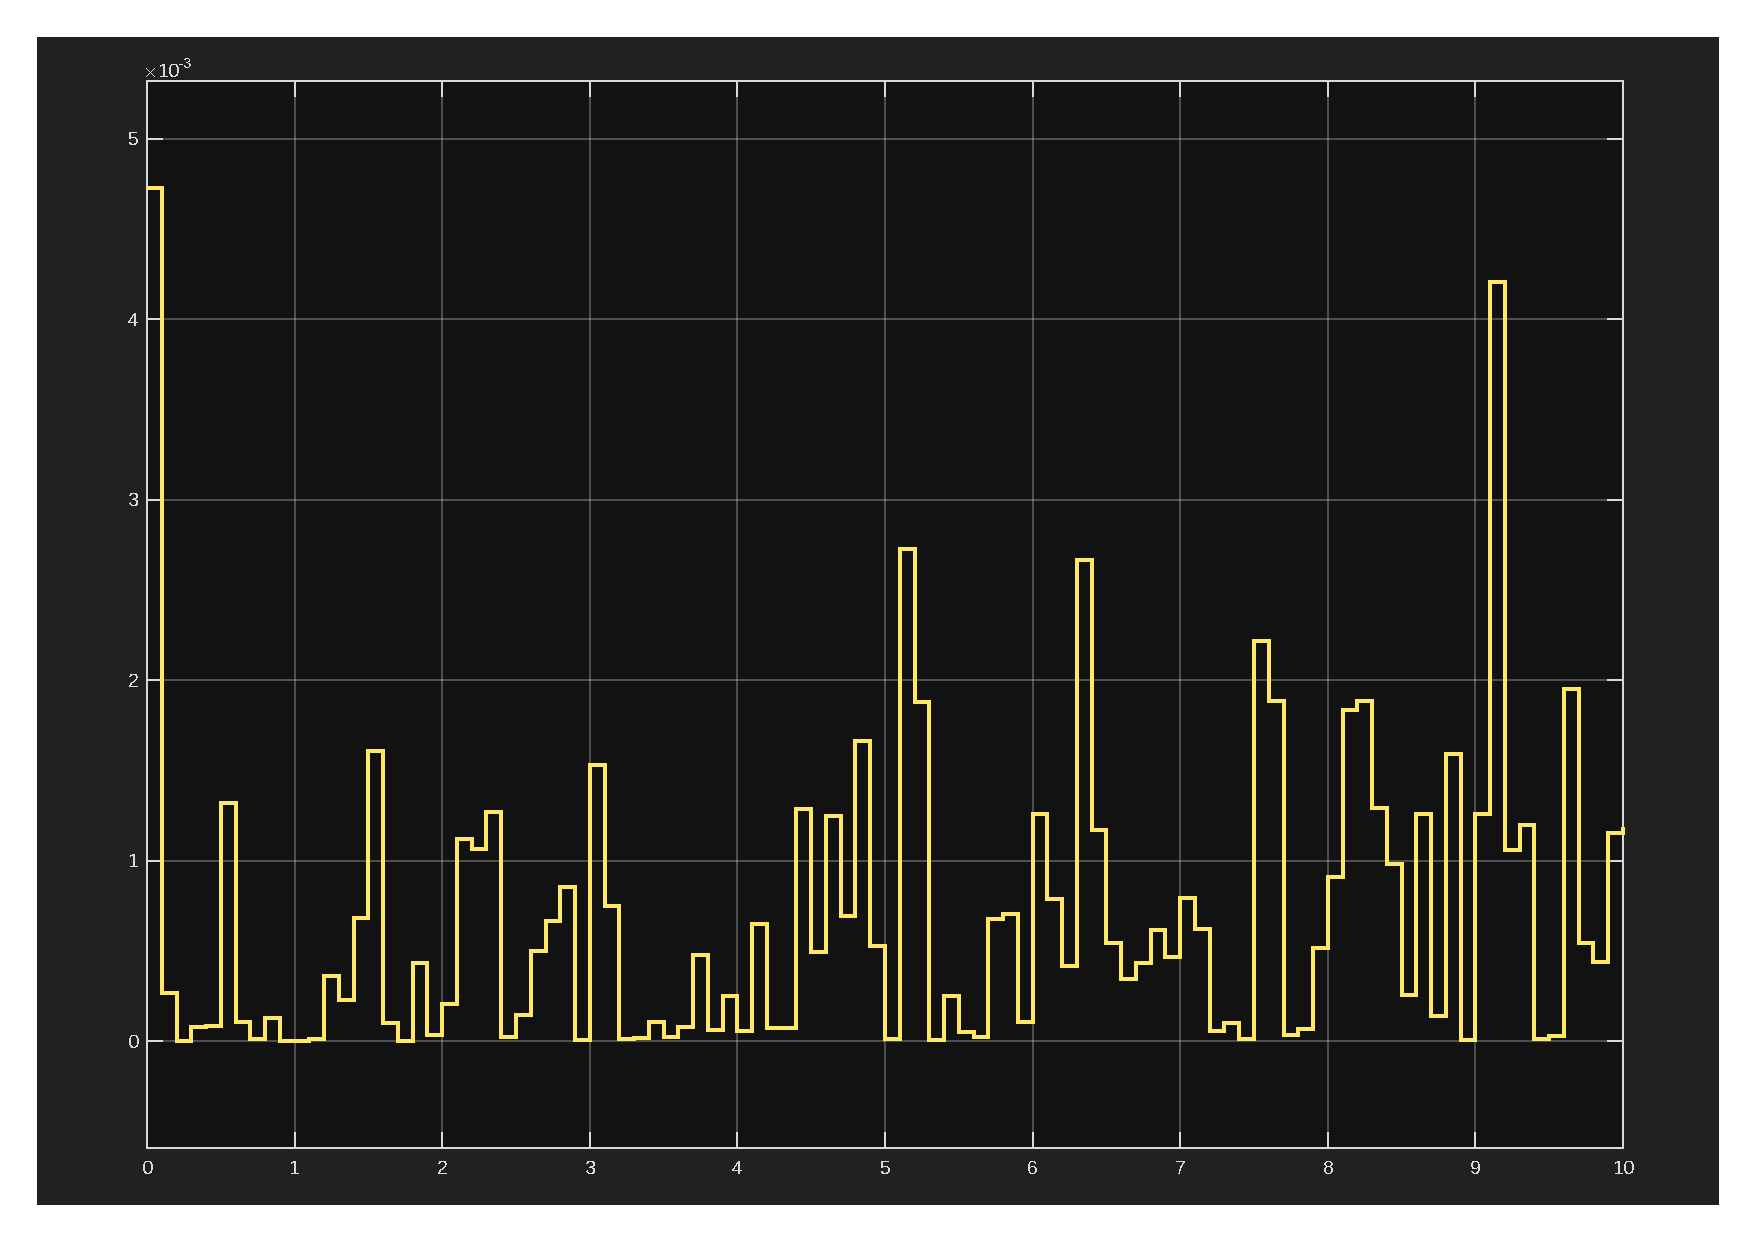
\includegraphics[width=\textwidth]{img/IdealOTA_MSE_simulink.pdf}
            \caption{Mean Square Error of the ideal OTA computation network over an \gls{awgn} channel.}
            \label{fig:simulink_MSE_ideal}
        \end{subfigure}
        \hfill
        \begin{subfigure}{0.39\textwidth}
            \centering
            % \includegraphics[width=\textwidth]{img/simulink_ideal_placeholder.png}
            \framebox{
                \parbox{\textwidth}{
                    \centering \vspace{2cm} \textbf{Simulink Model Placeholder} \\ 
                    \small\textit{Insert screenshot of your Ideal Simulink model here.} 
                    \vspace{2cm}
                }
            }
            \caption{Simulink block diagram representing the ideal, unimpaired OTA computation network over an AWGN channel.}
            \label{fig:simulink_MSE_rc}
        \end{subfigure}
        \caption{Simulink MSEs}
        \label{fig:simulink_mse}
    \end{figure}

    % \begin{figure}[htpb]
    %     \centering
    %     \begin{tabular}{ccc}
    %         \videogriditem{0.31\textwidth}{video/E_Zmax1_027e2MHz.mkv}{E_Zmax1_027e2MHz.png} &
    %         \videogriditem{0.31\textwidth}{video/E_Zmax1_077e2MHz.mkv}{E_Zmax1_077e2MHz.png} &
    %         \videogriditem{0.31\textwidth}{video/E_Zmax1_127e2MHz.mkv}{E_Zmax1_127e2MHz.png} \\[1ex]
    %         
    %         \videogriditem{0.31\textwidth}{video/E_Zmax2_027e2MHz.mkv}{E_Zmax2_027e2MHz.png} &
    %         \videogriditem{0.31\textwidth}{video/E_Zmax2_077e2MHz.mkv}{E_Zmax2_077e2MHz.png} &
    %         \videogriditem{0.31\textwidth}{video/E_Zmax2_127e2MHz.mkv}{E_Zmax2_127e2MHz.png} \\
    %     \end{tabular}
    %     \caption{Electrical Field for 2.7, 7.7, and 12.7 GHz $Z_{max}$.}
    %     \label{img:E}
    % \end{figure}

    \subsection{GNU Radio Validation}
    Finally, the ideal model is verified using a \gls{sdr} environment
    in GNU Radio. To maintain the ideal conditions mathematically defined in (\ref{eq:mac_sum}),
    the Root Raised Cosine (RRC) filters are perfectly matched. Specifically, the
    interpolation rate at the transmitters and the decimation rate at the receiver are
    identically matched to the symbol design rate (\texttt{sps\_actual = sps\_design =
    6}). In other words the upsampling rate of the \gls{fir} filters matches the spacing between
    sample generation.

    An important architectural consideration emerges from the GNU Radio implementation: in the absence of explicit 
    digital modulation schemes, strategic downsampling at the transmitter becomes mandatory to enable proper filter 
    operation. Specifically, each individual sensor transmits one symbol while simultaneously discarding sixteen 
    interpolated samples, thereby maintaining compliance with Nyquist sampling criterion while leveraging the 
    spectral efficiency benefits of pulse shaping.

    \begin{figure}[htpb]
        \centering
        \includegraphics[width=\linewidth]{flowgraphs/idealOTA_grc.pdf}

        \caption{GNU Radio flowgraph for the ideal, Nyquist-compliant scenario.}
        \label{fig:grc_ideal}
    \end{figure}

    Under these constraints, the Eye Diagram remains perfectly "open" at the optimal
    sampling phase, and the Constellation Diagram exhibits tightly clustered points. The
    absence of horizontal dispersion in the constellation confirms that, prior to the
    introduction of timing offsets or Faster-Than-Nyquist signaling, the \gls{mac} superposition
    principle flawlessly computes the arithmetic average of the agricultural sensors.

    \begin{figure}[htpb]
        \centering
        \includegraphics[width=\linewidth]{img/IdealOTA.png}

        \caption{GNU Radio Eye \& Constelation Diagram for the ideal, Nyquist-compliant scenario.}
        \label{fig:grc_ideal_diagram}
    \end{figure}

    A critical implementation detail warranting emphasis concerns the optimal sampling phase selection. Empirical 
    observation from the GNU Radio receiver indicates that maximum data recovery is achieved at a sampling phase 
    offset of $33$ samples out of the $96$-sample cycle (\footnote{The fundamental cycle spans 16 symbols; with 
    6 samples per symbol, the total cycle length is $16 \times 6 = 96$ samples.}). This phase offset reflects 
    the group delay inherent to the polyphase interpolating and decimating \gls{fir} filter implementations, 
    necessitating careful calibration for optimal demodulation performance.
    
    \ifSubfilesClassLoaded{
        \clearpage
        \printbibliography
    }{}
\end{document}